\documentclass[6pt,letter]{article}\usepackage[]{graphicx}\usepackage[]{color}
% maxwidth is the original width if it is less than linewidth
% otherwise use linewidth (to make sure the graphics do not exceed the margin)
\makeatletter
\def\maxwidth{ %
  \ifdim\Gin@nat@width>\linewidth
    \linewidth
  \else
    \Gin@nat@width
  \fi
}
\makeatother

\definecolor{fgcolor}{rgb}{0.345, 0.345, 0.345}
\newcommand{\hlnum}[1]{\textcolor[rgb]{0.686,0.059,0.569}{#1}}%
\newcommand{\hlstr}[1]{\textcolor[rgb]{0.192,0.494,0.8}{#1}}%
\newcommand{\hlcom}[1]{\textcolor[rgb]{0.678,0.584,0.686}{\textit{#1}}}%
\newcommand{\hlopt}[1]{\textcolor[rgb]{0,0,0}{#1}}%
\newcommand{\hlstd}[1]{\textcolor[rgb]{0.345,0.345,0.345}{#1}}%
\newcommand{\hlkwa}[1]{\textcolor[rgb]{0.161,0.373,0.58}{\textbf{#1}}}%
\newcommand{\hlkwb}[1]{\textcolor[rgb]{0.69,0.353,0.396}{#1}}%
\newcommand{\hlkwc}[1]{\textcolor[rgb]{0.333,0.667,0.333}{#1}}%
\newcommand{\hlkwd}[1]{\textcolor[rgb]{0.737,0.353,0.396}{\textbf{#1}}}%
\let\hlipl\hlkwb

\usepackage{framed}
\makeatletter
\newenvironment{kframe}{%
 \def\at@end@of@kframe{}%
 \ifinner\ifhmode%
  \def\at@end@of@kframe{\end{minipage}}%
  \begin{minipage}{\columnwidth}%
 \fi\fi%
 \def\FrameCommand##1{\hskip\@totalleftmargin \hskip-\fboxsep
 \colorbox{shadecolor}{##1}\hskip-\fboxsep
     % There is no \\@totalrightmargin, so:
     \hskip-\linewidth \hskip-\@totalleftmargin \hskip\columnwidth}%
 \MakeFramed {\advance\hsize-\width
   \@totalleftmargin\z@ \linewidth\hsize
   \@setminipage}}%
 {\par\unskip\endMakeFramed%
 \at@end@of@kframe}
\makeatother

\definecolor{shadecolor}{rgb}{.97, .97, .97}
\definecolor{messagecolor}{rgb}{0, 0, 0}
\definecolor{warningcolor}{rgb}{1, 0, 1}
\definecolor{errorcolor}{rgb}{1, 0, 0}
\newenvironment{knitrout}{}{} % an empty environment to be redefined in TeX

\usepackage{alltt} 

%%%%%%%%%%%%%%%%%%%%
%%%%%% Package %%%%%
%%%%%%%%%%%%%%%%%%%%

%\usepackage[latin1]{inputenc}
\usepackage[parfill]{parskip} % Activate to begin paragraphs with an empty line rather than an indent
\usepackage{amsmath,amsthm,amssymb,bbm} %math stuff
\usepackage{placeins} % FloatBarrier
\usepackage{fancyhdr}
\usepackage{lastpage}
\usepackage{float}    % for fig.pos='H'
\usepackage{rotfloat} % for sidewaysfigure
%\usepackage{subfig}   % for subfigure
\usepackage{subcaption}  % an alternative package for sub figures
\usepackage{comment}
\bibliographystyle{plainnat}
\usepackage{setspace} %Spacing
\usepackage{graphicx,graphics}
\usepackage{booktabs,tabularx}
\usepackage{enumerate}
\usepackage{makecell}
\usepackage{xfrac}
\restylefloat{figure}
\usepackage{appendix}
\usepackage{color, colortbl, xcolor}
\usepackage{booktabs,dcolumn} % for use with texreg in R
\usepackage[bookmarks]{hyperref}
\usepackage[backend=bibtex]{biblatex}
\usepackage{wrapfig}
\usepackage{todonotes}
\usepackage{ctable}
\usepackage{acronym}


%%%%%%%%%%%%%%%%%%%%%%%%%
%%%%%% Configuration %%%%
%%%%%%%%%%%%%%%%%%%%%%%%%
\bibliography{global}

\newcommand{\nd}{\noindent}
\newcommand{\ntodo}[2][]{\todo[#1]{\thesubsubsection{}. #2}}

% Define the format of the report
\renewcommand{\headrulewidth}{0.0pt}
\renewcommand{\footrulewidth}{0.0pt}
\setlength{\textheight}{9.00in}
\setlength{\textwidth}{7.00in}
\setlength{\topmargin}{-0.5in}
\setlength{\evensidemargin}{-0.25in}
\setlength{\oddsidemargin}{-0.25in}
\renewcommand{\baselinestretch}{1.2}
\makeatletter
\makeatother
\lfoot{} \cfoot{ } \rfoot{{\small{\em Page \thepage \ of \pageref{LastPage}}}}

\newenvironment{conditions}
  {\par\vspace{\abovedisplayskip}\noindent\begin{tabular}{>{$}l<{$} @{${}={}$} l}}
  {\end{tabular}\par\vspace{\belowdisplayskip}}
%%%%%%%%%%%%%%%%%%%%%%%%%%%%%%%%%%%%%%%%%%%%%%%%%%%
%%%%%%%%%%%%%%%%% BEGIN        %%%%%%%%%%%%%%%%%%%%
%%%%%%%%%%%%%%%%%%%%%%%%%%%%%%%%%%%%%%%%%%%%%%%%%%%
\IfFileExists{upquote.sty}{\usepackage{upquote}}{}
\begin{document}
\pagestyle{plain}
\pagenumbering{gobble}

\title{%
 Méthodes avancées en exploitation de donnée \\
  \large (MATH80619)}
\author{\begin{tabular}{ll}
    Estefan Apablaza-Arancibia & 11271806\\
        Adrien Hernandez & 11269225\\

    
\end{tabular}}
\maketitle
\newpage
\pagestyle{plain}
\section*{List of Acronyms}
\begin{acronym}
\acro{API}{Application Programming Interface} 
\acro{CNN}{Convulutional Neural Network} 
\acro{FNN}{Feed-Forward Neural Network} 
\acro{RNN}{Recurent Neural Network} 

\end{acronym} 

%%%%%%%%%%%%%%%%%%%%%%%%%%%%%%%%%%%%%%%%%%%%%%%%%%%
%%%%%%%%%%%%%%%%% INTRODUCTION %%%%%%%%%%%%%%%%%%%%
%%%%%%%%%%%%%%%%%%%%%%%%%%%%%%%%%%%%%%%%%%%%%%%%%%%
\newpage
\pagestyle{fancy}
\pagenumbering{arabic}
\section{Introduction}
In the first section of this paper, a literature review covers the neural networks and deep learners algorithms, focusing on different type of neural networks architecture; the purpose of adding multiple hidden layers and, ultimately, what are the challenges regarding the increase in computing time. Furthermore, in the methodology section, a list of deep learning projects are shown in order to understand some patterns and methods. Then, an exhaustive list of the R libraries allowing to build neural networks and deep learners models. Correspondingly, the advantages and disadvantages of each libraries, their capabilities as well as what you can expect when using them. To sum up, the last section will give concrete examples on how to implement the neural networks and deep learners models with these libraries, using real data.

%%%%%%%%%%%%%%%%%%%%%%%%%%%%%%%%%%%%%%%%%%%%%%%%%%%
%%%%%%%%%%%%%%%%%% Litterature %%%%%%%%%%%%%%%%%%%%
%%%%%%%%%%%%%%%%%% Review      %%%%%%%%%%%%%%%%%%%%
%%%%%%%%%%%%%%%%%%%%%%%%%%%%%%%%%%%%%%%%%%%%%%%%%%%

\section{Litterature Review}
\subsection{What is Deep Learning and why use it?}
\begin{wrapfigure}[14]{r}{0.5\textwidth}
  \begin{center}
    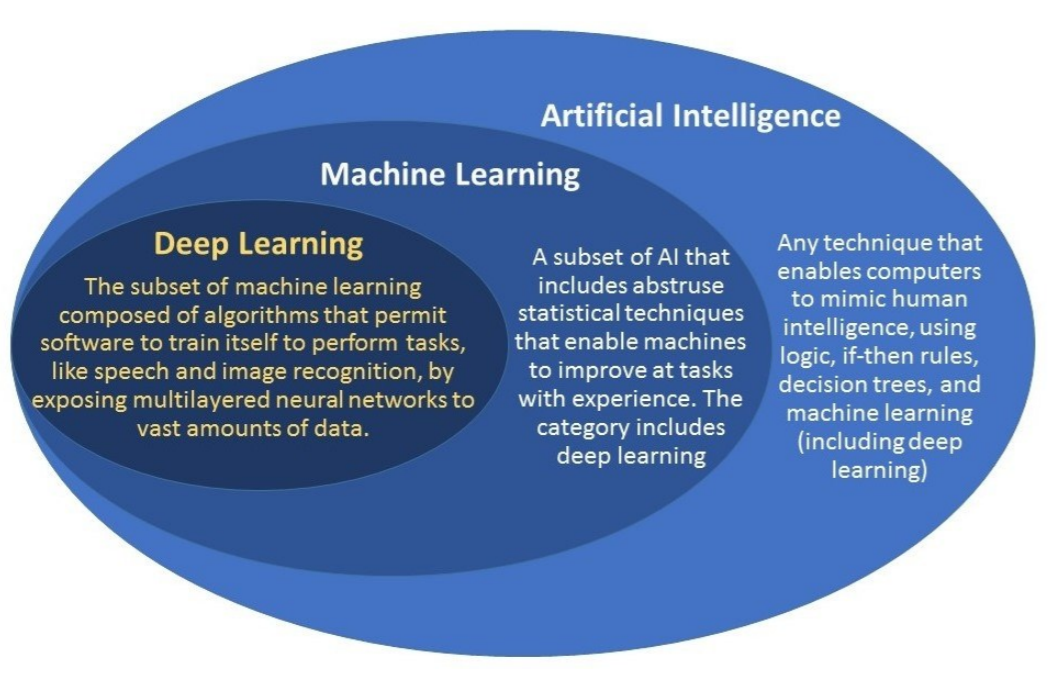
\includegraphics[width=0.4\textwidth]{deep learning.PNG}
      \end{center}
     \caption{Artificial Intelligence vs Machine Learning vs Deep Learning}
     \label{fig:simule}
\end{wrapfigure}

Deep learning is a subset field of articial intelligence and can be seen as a specific way of doing machine learning. Deep learning algorithms can be seen as feature representation learning. Indeed, by applying to the data multiple non-linear transformations through the use of hidden layers, deep learning models have their own trainable feature extration capability making it possible to learn specific features from the data without needing a specific human domain expert. This means that deep learning models won't require the features extraction step that is essential for classic machine learning models. However, increasing the models capacity by adding hidden layers, requires increasingly computing power and slow down the training process of the model. The choice of hyperparameters, programming languages and memory management will therefore be important criteria to take into account will building deep learning models\\
Since the last decade, deep learning models have shown notable predictive power and have been revolutionizing an important number of domain such as computer vision, natural language understanding, fraud detection, health and much more.\\
As a first glance in the subject, it is highly recommended it to read  a reference from pioneers in the field (\cite[Chapter 1]{Goodfellow-et-al-2016}).


\subsubsection{Feed Forward Neural Network}
\begin{wrapfigure}[12]{R}{0.5\textwidth}
  \begin{center}
    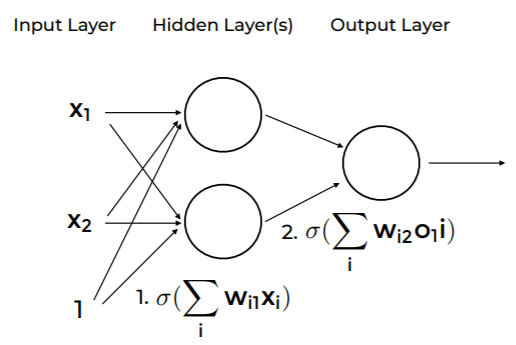
\includegraphics[width=0.4\textwidth]{feedforward_neural_networks.png}
  \end{center}
  \caption{feedforward neural networks}
  \label{fig:attention}
\end{wrapfigure}

"Deep feedforward networks, also called feedforward neural networks, or multilayer perceptrons (MLPs), are the quintessential deep learning models." \cite{Goodfellow-et-al-2016}

\ac{FNN} models are inspired from biology and by the way the human brain works. In a neural network, each neuron takes input from other neurons, processes the information and then transmits outputs to next neurons. Artificial neural networks follow the same process as each neuron will perform the weighted sum of inputs and will add a bias as a degree of freedom. It will then apply a non-linear transformation before outputting the information. Thus, the information goes forward in the network; neurons transmit information from the input layers towards the output layer. It is important to know that in a feedfoward neural networks (fig. \ref{fig:attention}) the neurons of a same layer are not connected to each other; they do not allow any feedback connections within a same layer. If we want to allow this process, we will be looking at recurrent neural networks.

The equation a neuron input is  
\begin{equation}
a(x) = b +\sum_{i}{w_i x_i}
\end{equation}
and the output
\begin{equation}
h(x) = g(a(x))
\end{equation}
where:
\begin{conditions}
 x     &  the input data \\
 b     &  the bias term \\
 w     &  the weight or parameter \\   
 g(...) &  the activation function
\end{conditions}
A detailed explanation of the theory of feedforward neural network can be found in \cite[Chapter 6]{Goodfellow-et-al-2016}


\subsubsection{\ac{CNN}}
The \ac{CNN} are a modified architeturce of \ac{FNN} that leverage the feature engineering that use to be hand maded by domain experts. This class of deep neural network are commonly use for image recognition and classification that can serve different application such as facial recongnition, document analysis and speech recognition. The original \ac{FNN} are not suited analyzing large size images since the weights increase exponentially and ,at the end, don't perfom very well. To get a detailed explanation of convolutional neural networks we recommand to read \cite[Chapter 9]{Goodfellow-et-al-2016}.
\subsubsection{RNN}
Recurrent neural networks are a type of neural networks architecture having proven state-of-art performance for solving tasks related to sequential data such as Natural Language Processing (NLP), anomaly detection and event forecasting. As a key differentiator from feedfoward neural networks, they include feedback loops connections and get an internal memory. One of their other advantage is to be able to handle input and ouput sequences with different 
To get a detailed explanation of the theory of recurrent neural networks we recommand to read \cite[Chapter 10]{Goodfellow-et-al-2016}.

\subsection{How to integrate Deep Learning in R}
The integration of Deep learning in R can be separate in two part ; (1) The \ac{API} integration and (2) the standalone R packages. 
\begin{enumerate}
\item The \ac{API} will give the possibility to control externally through R an existing installation. In other words, a software translator for a already known software installation. This approach is not always trivial to install nor to manipulate but in long term will probably give the best flexibility in terms of Deep Learning projects.
\item The standalone R packages will be packages that require no third party software in order to create the deep learning projects. This approach is relatively fast to install but is restraing in terms deep learning architecture.
\end{enumerate}
A list of the available resources with installation and examples tutorials can be found in section \ref{avail_ressour} and \ref{examples} .
%%%%%%%%%%%%%%%%%%%%%%%%%%%%%%%%%%%%%%%%%%%%%%%%%%%
%%%%%%%%%%%%%%%%%% Description %%%%%%%%%%%%%%%%%%%%
%%%%%%%%%%%%%%%%%% of methods  %%%%%%%%%%%%%%%%%%%%
%%%%%%%%%%%%%%%%%%%%%%%%%%%%%%%%%%%%%%%%%%%%%%%%%%%

\section{Description of methods}
\ntodo[inline]{I think this section is more to explain, for example, the dataset with their end objective so when we are doing examples we just say we are going to use the CIFAR10 and the readers know we are doing a classification problem.}

\section{Methodology}
\ntodo[inline]{Give example of deep learning project pocedure}

%%%%%%%%%%%%%%%%%%%%%%%%%%%%%%%%%%%%%%%%%%%%%%%%%%%
%%%%%%%%%%%%%%%%%% Resources   %%%%%%%%%%%%%%%%%%%%
%%%%%%%%%%%%%%%%%% available   %%%%%%%%%%%%%%%%%%%%
%%%%%%%%%%%%%%%%%%%%%%%%%%%%%%%%%%%%%%%%%%%%%%%%%%%

\section{Available resources}
\label{avail_ressour}
\ntodo[inline]{Très intéressant:\url{https://edu.kpfu.ru/pluginfile.php/419285/mod_resource/content/2/neural-networks-r.pdf}}
\ntodo[inline]{Faire une recherche exhaustive des ressources disponibles en R pour faire des analyses liées à ce sujet. Par exemple: fonctions R de base, packages sur les différentes plate-formes (CRAN, )}
According to the CRAN-R project website, we give a list of the different packages known in R allowing to use simple and deep neural network algorithms. \newline \url{https://cran.r-project.org/web/views/MachineLearning.html}



\subsection{\ac{API} packages}
\subsubsection{Keras}
\paragraph{How to install it}
\ntodo[inline]{Très très intéressant:\url{https://r2018-rennes.sciencesconf.org/data/pages/Deep_with_R_1.pdf}}
First step, is the installation and download of the Keras files from GitHub :
\begin{knitrout}
\definecolor{shadecolor}{rgb}{0.969, 0.969, 0.969}\color{fgcolor}\begin{kframe}
\begin{alltt}
\hlstd{devtools}\hlopt{::}\hlkwd{install_github}\hlstd{(}\hlstr{"rstudio/keras"}\hlstd{)}
\end{alltt}
\end{kframe}
\end{knitrout}
Then, we need to to install the package and import in the project :
\begin{knitrout}
\definecolor{shadecolor}{rgb}{0.969, 0.969, 0.969}\color{fgcolor}\begin{kframe}
\begin{alltt}
\hlkwd{library}\hlstd{(keras)}
\hlkwd{install_keras}\hlstd{()}
\end{alltt}
\begin{verbatim}
## 
## Installation complete.
\end{verbatim}
\end{kframe}
\end{knitrout}
When the "\textit{Installation complete.}" message appear you have a complete installation with CPU configure on the TensorFlow backend.
If you want to take advantage of your GPU (Ensure that you have the hardware prerequisites) you will need to execute a different command as follows:
\begin{knitrout}
\definecolor{shadecolor}{rgb}{0.969, 0.969, 0.969}\color{fgcolor}\begin{kframe}
\begin{alltt}
\hlkwd{install_keras}\hlstd{(}\hlkwc{tensorflow} \hlstd{=} \hlstr{"gpu"}\hlstd{)}
\end{alltt}
\end{kframe}
\end{knitrout}

\paragraph{Tensorflow backend}


\paragraph{CNTK backend}
\paragraph{Theano backend}

%$https://keras.rstudio.com/$
\subsubsection{Tensorlow}

\subsubsection{rTorch}

\subsection{R packages}

\subsubsection{RSNNS}

Another package \textbf{RSNNS} (Bergmeir, 2019) allows to have access to a high view of the pakcage SNNS (Stuttgart Neural Network Simulator), containing several neural networks algorithms \ntodo[inline]{à creuser ce package}

\subsubsection{Deepnet}

For deep learning algorithms, \textbf{Deepnet} (Rong, 2014), allows to us neural networks with several hidden layers. This package contains interesting features such as neural networks having their neurones' weight automatically initialized by a DBN (deep belief network) or a stacked autoencoder. (\ntodo[inline]{il fait aussi Boltzmann machine, à voir ce que c'est})\\

Another package, \textbf{RcppDL} (Kou and Sugomori, 2014), allows a simple use of deep neural netowkrsm including denoising autoencoders, stacked denoising autoencoder, restricted Boltzmann machines and deep belief nets.\\

\subsubsection{H2o} (LeDell, 2020) video qui explique h2o 
%$https://www.youtube.com/watch?v=g7drhm_SdbQ$
H2o is a "scalable open source machine learning platform that offers parallelized implementations of many supervised, unsupervised and fully automatic machine learning algorithms on clusters". This package allows to run H2o via its REST API through R and offers several advantages such as the ability ot know the computation time remaining when running a model.
Prerequisites to launch H2o, 64 bit Java 6+ if you want to open a h2o model that s more than 1 GB. 
R users: prerequisite R installed. Add R to your PATH. install.packages("h2o")
different syntax to work with h2o. read.csv = h2o.importFile. cbind = h2o.cbind. predict = h2o.predict. glm = h2o.glm, ...
According to KD Nuggets, "Recurrent Neural Networks and Convolutional Neural Networks can be constructed using H2o's deep water project throught others libraries such as Caffe and TensorFlow". "Some of the features of H2o deep learning models are: Automatic Adaptive learning rate, Model regularization, Model checkpointing, Grid Search". Source: 
%https://www.kdnuggets.com/2018/01/deep-learning-h2o-using-r.html
$a(x) = b +\sum_{i}{w_i x_i}$

\ntodo[inline]{Faire une recherche exhaustive des ressources disponibles en R pour faire des analyses liées à ce sujet. Par exemple: fonctions R de base, packages sur les différentes plate-formes (CRAN, )}
According to the CRAN-R project website, we give a list of the different packages known in R allowing to use simple and deep neural network algorithms. \newline \url{https://cran.r-project.org/web/views/MachineLearning.html}
\subsubsection{Nnet} (Ripley and Venables, 2016) allows to quickly train and fit a feed-forward neural networks with one hidden layer. This package does not allow to use more that one hidden layer, and does not have any feature to find the optimal number of neurones in the hidden layer. It is up to the analyst to build a loop to test by cross-validation, for exemple, the optimal hyperparameter values.\url{https://cran.r-project.org/web/packages/nnet/nnet.pdf}\\


\subsubsection{brnn}

\subsubsection{deepnlp}


\subsubsection{neuralnet} allows to plot the neural net (keras allows it too i think)

\ntodo[inline]{Ce mec parle de la gestion de la memoire en R avec keras, qui me semble utilise des numpy array en backend ... à creuser mais peut etre interessant d'en parler car le gros probleme de R pour le deep learning c'est sa gestion de la memoire }
\url{https://community.rstudio.com/t/deep-learning-in-r-memory-allocation/17541}

\ntodo[inline]{Bonne ressource pour videos \url{https://www.youtube.com/user/westlandindia/videos}}
\begin{table}
\centering
\begin{tabular}{lllll}
Package      & Pro & Con & Actif & URL   \\
tensorflow R &     &     &       & Link  \\
Kera R       &     &     &       &       \\
MxNet        &     &     &       &      
\end{tabular}
\end{table}
\ntodo[inline]{Ici on pourrait faire un tableau avec tous les packages et donner les pour et les contres, ADRIEN: Le tableau je suis pas trop fan sachant qu on doit ecrire 20 pages sur ces librairies}

%%%%%%%%%%%%%%%%%%%%%%%%%%%%%%%%%%%%%%%%%%%%%%%%%%%
%%%%%%%%%%%%%%%%%% Examples    %%%%%%%%%%%%%%%%%%%%
%%%%%%%%%%%%%%%%%%%%%%%%%%%%%%%%%%%%%%%%%%%%%%%%%%%
\section{Examples}
\label{examples}
\ntodo[inline]{Encore à voiron pourrait créer des tutoriels pour peut-être comparer}
\ntodo[inline]{Il faut trouver des datasets intéressantes à utiliser avec les differents packages}


\FloatBarrier 
\clearpage 
\pagestyle{plain}
\ntodo[inline]{Find a way to remove page number from references}

\printbibliography



\end{document}
